\begin{frame}
  \begin{center}
    \Large{Machine learning}
  \end{center}
\end{frame}

\begin{frame}
  \begin{center}
    \includegraphics[scale=0.45]{./pictures/polynomials.png}
  \end{center}
\end{frame}

% TODO ? graph with pictures of digits on the x-axis and their corresponding digit
% on the y-axis

\begin{frame}
  \begin{center}
    \begin{tikzpicture}[]

      % horizontal axis
      \draw[->] (0,0) -- (5,0) node[anchor=north] {};
      \draw   (0.5,0) node[anchor=north] {\includegraphics[scale=0.2]{./pictures/0.png}}
      (1.0,0) node[anchor=north] {\includegraphics[scale=0.3]{./pictures/1.png}}
      (1.5,0) node[anchor=north] {\includegraphics[scale=0.3]{./pictures/2.png}}
      (2.0,0) node[anchor=north] {\includegraphics[scale=0.3]{./pictures/3.png}}
      (2.5,0) node[anchor=north] {\includegraphics[scale=0.3]{./pictures/4.png}}
      (3.0,0) node[anchor=north] {\includegraphics[scale=0.3]{./pictures/5.png}}
      (3.5,0) node[anchor=north] {\includegraphics[scale=0.3]{./pictures/6.png}}
      (4.0,0) node[anchor=north] {\includegraphics[scale=0.3]{./pictures/7.png}}
      (4.5,0) node[anchor=north] {\includegraphics[scale=0.3]{./pictures/8.png}}
      (5.0,0) node[anchor=north] {\includegraphics[scale=0.3]{./pictures/9.png}};

      % horizontal axis
      \draw[->] (0,0) -- (0,5) node[anchor=north] {};
      \draw (0,0.5) node[anchor=east] {0}
      (0,1.0) node[anchor=east] {1}
      (0,1.5) node[anchor=east] {2}
      (0,2.0) node[anchor=east] {3}
      (0,2.5) node[anchor=east] {4}
      (0,3.0) node[anchor=east] {5}
      (0,3.5) node[anchor=east] {6}
      (0,4.0) node[anchor=east] {7}
      (0,4.5) node[anchor=east] {8};
      (0,5.0) node[anchor=east] {9};

      \node (?) at (2.5, 2.5) {?};

    \end{tikzpicture}
  \end{center}
\end{frame}

% TODO feed-forward neural network graph
\begin{frame}
  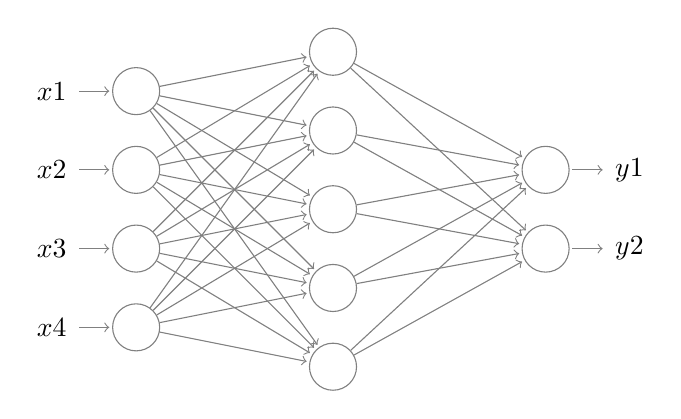
\begin{tikzpicture}[shorten >=1pt,->,draw=black!50, node distance=2.5cm]
    \tikzstyle{every pin edge}=[<-,shorten <=1pt]
    \tikzstyle{neuron}=[circle,draw,minimum size=17pt,inner sep=0pt]

    % input layer nodes
    \foreach \y in {1,...,4}
    \node[neuron, pin=left:$x\y$] (I-\y) at (0,-\y) {};

    % hidden layer nodes
    \foreach \y in {1,...,5}
    \path[yshift=0.5cm]
    node[neuron] (H-\y) at (2.5,-\y) {};

    % output layer node
    \foreach \y in {1,2}
    \path[yshift=-1cm]
    node[neuron,pin={[pin edge={->}]right:$y\y$}, right of=H-2] (O-\y) at (2.7,-\y) {};

    % Connect every node in the input layer with every node in the
    % hidden layer.
    \foreach \src in {1,...,4}
    \foreach \dst in {1,...,5}
    \path (I-\src) edge (H-\dst);

    % Connect every node in the hidden layer with the output layer
    \foreach \src in {1,...,5}
    \foreach \dst in {1,2}
    \path (H-\src) edge (O-\dst);
  \end{tikzpicture}
\end{frame}
